\documentclass[10pt,a4paper]{article}
\usepackage[T1]{fontenc}
\usepackage[utf8]{inputenc}
\usepackage{lmodern}
\usepackage[margin=1.6cm,top=2.3cm,bottom=1.8cm,headheight=28pt]{geometry}
\usepackage{graphicx,booktabs,array,tabularx,longtable,amsmath,amssymb,xcolor,float,fancyhdr,enumitem,url}
\usepackage[hidelinks]{hyperref}
\setlength{\parindent}{0pt}\setlength{\parskip}{3pt}
\definecolor{hdr}{HTML}{E8EEF5}
\pagestyle{fancy}\fancyhf{}
\fancyhead[L]{\footnotesize \copyright\,VIT IPR\&TT CELL}
\fancyhead[C]{\footnotesize\textbf{Invention Disclosure Format (IDF)-B}}
\fancyhead[R]{\footnotesize Doc.\ No.\ 02-IPR-R003\\ Issue No/Date 2/01.02.2024\\ Amd.\ No/Date 0/00.00.0000}
\fancyfoot[C]{\footnotesize Page \thepage}
\newcommand{\sect}[1]{\par\vspace{5pt}{\bfseries\large #1}\par\vspace{1pt}}
\newcolumntype{L}[1]{>{\raggedright\arraybackslash}p{#1}}
\begin{document}

\sect{1. Title of the invention}
\textbf{Method and System for Energy-Optimal, Risk-Bounded Autonomous Actuation in Ambient-Intelligence IoT Using a Conformal Sensing Cascade with Optimised Risk-Budget Allocation (AmI-CC)}

\sect{2. Field / Area of invention}
Ambient Intelligence (AmI) for AI-native Internet of Things; context-aware multimodal sensing; energy-efficient edge AI; trustworthy (statistically guaranteed) autonomous actuation in smart homes, buildings, assisted living and Industry~5.0. Responds to the IEEE Internet of Things Journal special issue on ``Ambient Intelligence for AI-Native IoT: Invisible, Context-Aware, and Autonomous Experiences'' (topics: AmI architectures, context-aware sensing, edge AI, explainable/trustworthy AmI, energy-efficient AI-native IoT).

\sect{3. Prior patents and publications from literature}
\footnotesize
\begin{longtable}{@{}L{0.6cm}L{4.6cm}L{4.2cm}L{7.6cm}@{}}
\toprule \textbf{\#} & \textbf{Reference (verify before filing)} & \textbf{What it teaches} & \textbf{Gap vs.\ present invention}\\ \midrule \endhead
1 & US 9,159,208, ``Energy efficient cascade of sensors for automatic presence detection'' (USPTO) & Cascade of sensors; cheaper sensors gate costlier ones to save power. & Gate is heuristic/threshold based; no distribution-free bound on wrong actuation; no budget split; no deferral semantics.\\
2 & Angelopoulos, Bates, Fisch, Lei, Schuster, ``Conformal Risk Control'', ICLR 2024 (arXiv:2208.02814) & Calibrating a single threshold to bound expected monotone loss. & Single model/stage; not a multi-sensor, energy-costed cascade; no allocation of a global budget across stages.\\
3 & ``Fast yet Safe: Early-Exiting with Risk Control'', arXiv:2405.20915 & Risk-controlled early exit in neural networks. & Exits inside one network (compute saving); does not power physical sensor tiers; no energy-optimal per-tier budget split; no actuate/escalate/defer policy.\\
4 & ``Efficient Conformal Prediction via Cascaded Inference with Expanded Admission'', arXiv:2007.03114 & Cascaded models to cheapen conformal sets. & Model cascade for set size; no sensing-hardware wake-up; no actuation risk.\\
5 & Gibbs \& Cand\`es, ``Adaptive Conformal Inference Under Distribution Shift'', NeurIPS 2021 & Online adaptation of miscoverage level under shift. & Generic; not applied to per-tier budgets of a sensing cascade.\\
6 & Jitkrittum et al., ``When Does Confidence-Based Cascade Deferral Suffice?'', NeurIPS 2023 (arXiv:2307.02764) & Analysis of confidence-threshold deferral in model cascades. & Heuristic confidence rules, no finite-sample guarantee (our baseline behaves this way).\\
7 & ``Sensor-Aware Classifiers for Energy-Efficient Time Series Applications on IoT Devices'', arXiv:2407.08715 & Early-exit classifiers exploiting sensor structure for energy. & No statistical guarantee on wrong decisions; no joint budget allocation.\\
8 & ``Early Time Classification with Accumulated Accuracy Gap Control'', arXiv:2402.00857 & Stopping-time classification with accuracy-gap control. & Time-series stopping, not multi-tier hardware sensing; no energy-optimal allocation.\\
\bottomrule
\end{longtable}
\vspace{-6pt}{\scriptsize Note: a professional patent-database search (Espacenet, Google Patents, InPASS; CPC G06N~20/00, G16Y, H04W~52/02, G05B~13) must confirm this table before filing. References 1--8 were identified by web search on 30-Sep-2026; only titles/abstract-level content was reviewed.}
\normalsize

\sect{4. Summary and background of the invention (gap / novelty)}
\textbf{Background.} Ambient IoT must act \emph{invisibly} (no user prompts), yet a wrong autonomous action (unlocking a door, switching a heater, dismissing a fall alert) is costly, while always-on rich sensors (camera, mmWave radar) drain batteries and raise privacy exposure. Existing systems either (a) run all sensors and a single classifier (high energy; softmax confidence is uncalibrated), or (b) use heuristic confidence-threshold sensor cascades that give no assurance on how often they act wrongly, especially for unseen occupants.

\textbf{Gap.} No known system couples a \emph{physical sensing-tier wake-up cascade} with a \emph{finite-sample, distribution-free bound on wrong autonomous actuation} while \emph{choosing how that bound is spent across tiers to minimise energy}.

\textbf{Invention.} At each tier a split-conformal prediction set over candidate intents is computed. A singleton set triggers actuation and stops (higher-energy sensors stay asleep); a non-singleton set wakes the next tier; ambiguity at the last tier defers to the user (or a safe default). A wrong actuation implies the true intent was outside the stopping tier's set, so the wrong-actuation probability is bounded by the sum of per-tier miscoverage levels (union bound)---the \textbf{risk budget} $\alpha$. The novel \textbf{budget-allocation step} searches the split of $\alpha$ over tiers that minimises expected energy $+\lambda\cdot$deferral rate on one data split and calibrates the thresholds on a \emph{disjoint} split, so the guarantee stays valid. On-site recalibration with few labelled samples restores the bound under occupant shift.

\sect{5. Objective(s) of the invention}
(i) Bound the rate of erroneous autonomous actuation by an operator-set budget $\alpha$ without distributional assumptions; (ii) minimise sensing energy by waking high-power / privacy-intrusive modalities only when cheaper ones are ambiguous; (iii) provide a principled abstain (``ask user'') behaviour instead of forced decisions; (iv) make the guarantee portable to new occupants/homes through lightweight recalibration; (v) run on edge hardware (linear heads suffice; the allocation is a small grid search).

\sect{6. Working principle of the invention (in brief)}
Tier-$t$ score $s=1-p_t(y\mid x)$; threshold $q_t$ is the $\lceil (n+1)(1-\alpha_t)\rceil$-th smallest calibration score; set $C_t(x)=\{k:\,1-p_{t,k}(x)\le q_t\}$. Rule: $|C_t|=1\Rightarrow$ actuate and stop; otherwise escalate; last tier non-singleton $\Rightarrow$ defer. Then $P(\text{wrong actuation})\le\sum_t\alpha_t\le\alpha$. Allocation:
\[(\alpha_1,\dots,\alpha_T)^{*}=\arg\min\ \mathbb{E}[\text{energy}]+\lambda\,P(\text{defer})\quad\text{s.t.}\ \textstyle\sum_t\alpha_t\le\alpha,\]
solved by grid search on an allocation split; thresholds are calibrated on a disjoint split.

\sect{7. Description of the invention in detail}
\textbf{7.1 Architecture.} (a) Sensing tiers: T1 passive low-power (PIR, door contact, ambient light, time of day; 1 energy unit), T2 medium (plug power, audio level, BLE RSSI; 6 units), T3 high (camera / mmWave embedding; 40 units). (b) Per-tier classifiers over cumulative features (edge MCU / gateway). (c) Conformal calibrator storing per-tier score quantiles. (d) Budget allocator. (e) Actuation controller with escalate / actuate / defer outputs. (f) Optional on-site recalibration module fed by user overrides.

\textbf{7.2 Procedure.} \emph{Offline:} (1) train tier classifiers on training occupants; (2) on the allocation split run the cascade for each candidate split $(\alpha_1,\dots,\alpha_T)$ with $\sum_t\alpha_t=\alpha$ and keep the split minimising $J=\mathbb{E}[\text{cumulative energy}]+\lambda P(\text{defer})$; (3) on a disjoint calibration split compute $q_t$. \emph{Online:} power tier~1, compute the set; if singleton, actuate; otherwise power tier~2, and so on; at the last tier defer if not singleton.

\textbf{7.3 Why the bound holds.} If the cascade actuates wrongly at tier $t$ then $C_t=\{\hat y\}$ with $\hat y\neq y$, hence $y\notin C_t$; split-conformal prediction gives $P(y\notin C_t)\le\alpha_t$ under exchangeability; a union over tiers gives $\le\sum_t\alpha_t$. Because the allocation uses data disjoint from the calibration data, the $q_t$ remain valid.

\textbf{7.4 Implementation.} Reference implementation in Python (repository directories \texttt{amicg/} [simulator, cascade], \texttt{experiments/}, \texttt{tests/}; unit tests pass).

\begin{figure}[H]\centering\small
\begin{tabular}{@{}l c l@{}}
\toprule
Sensors T1 (1u) & $\rightarrow$ & Classifier$_1$ + conformal set $C_1$; $|C_1|=1$? yes $\to$ \textbf{ACTUATE} (stop)\\
\multicolumn{3}{c}{no $\downarrow$ wake T2 (6u)}\\
Sensors T2 (+6u) & $\rightarrow$ & Classifier$_2$ + set $C_2$; $|C_2|=1$? yes $\to$ \textbf{ACTUATE}\\
\multicolumn{3}{c}{no $\downarrow$ wake T3 (40u)}\\
Sensors T3 (+40u) & $\rightarrow$ & Classifier$_3$ + set $C_3$; $|C_3|=1$? yes $\to$ \textbf{ACTUATE}; no $\to$ \textbf{DEFER} to user\\
\bottomrule
\end{tabular}
\caption{Conformal sensing cascade. The budget allocator chooses $\alpha_1+\alpha_2+\alpha_3\le\alpha$; wrong actuation $\le\alpha$.}
\end{figure}

\sect{8. Experimental validation results}
\textbf{Setup (simulation; no real-deployment data yet).} Synthetic multi-tier smart-home benchmark with 8 intents (idle, enter home, cooking, TV, sleep, leave, exercise, fall-risk), 3 cumulative sensing tiers (6/14/26 features; energy 1/6/40 units), per-occupant offsets (inter-occupant covariate shift) and deliberately confusable intent pairs at low tiers. Per seed: 24 training occupants, 10 allocation, 14 calibration and 24 unseen test occupants, 150 samples each; 30 random seeds; means shown. Tier accuracies (single seed): T1 67\%, T2 80\%, T3 99.6\%. Baselines: always-all-sensors argmax; tier-1 only; single-stage conformal with always-full sensing; confidence-threshold cascade (single threshold tuned on the same calibration split to hit $\alpha$, forced decision at last tier); ablation: equal budget split.

\begin{table}[H]\centering\small
\caption{Main results, mean over 30 seeds (standard deviations in \texttt{results/results.json}). FA = false-actuation rate. Tier-1-only: FA $=0.330$, energy $=1$.}
\begin{tabular}{@{}c l c c c c@{}}
\toprule
$\alpha$ & Method & FA & Energy/decision & Deferral rate & Seeds with FA$>\alpha$\\ \midrule
0.01 & \textbf{AmI-CC (proposed)} & 0.0067 & 32.3 & 0.009 & 7\% \\
 & AmI-CC, equal split & 0.0043 & 33.6 & 0.003 & 0\% \\
 & Conformal, full sensing & 0.0011 & 47.0 & 0.009 & 0\% \\
 & Conf.-threshold cascade & 0.0109 & 31.7 & 0.000 & 57\% \\
 & All sensors, argmax & 0.0032 & 47.0 & 0.000 & 0\% \\
\midrule
0.02 & \textbf{AmI-CC (proposed)} & 0.0141 & 29.8 & 0.009 & 7\% \\
 & AmI-CC, equal split & 0.0073 & 31.9 & 0.005 & 0\% \\
 & Conformal, full sensing & 0.0005 & 47.0 & 0.020 & 0\% \\
 & Conf.-threshold cascade & 0.0196 & 29.2 & 0.000 & 50\% \\
 & All sensors, argmax & 0.0032 & 47.0 & 0.000 & 0\% \\
\midrule
0.05 & \textbf{AmI-CC (proposed)} & 0.0417 & 24.1 & 0.002 & 10\% \\
 & AmI-CC, equal split & 0.0164 & 28.9 & 0.014 & 0\% \\
 & Conformal, full sensing & 0.0002 & 47.0 & 0.051 & 0\% \\
 & Conf.-threshold cascade & 0.0481 & 23.6 & 0.000 & 47\% \\
 & All sensors, argmax & 0.0032 & 47.0 & 0.000 & 0\% \\
\midrule
0.1 & \textbf{AmI-CC (proposed)} & 0.0900 & 17.6 & 0.002 & 17\% \\
 & AmI-CC, equal split & 0.0359 & 25.0 & 0.023 & 0\% \\
 & Conformal, full sensing & 0.0001 & 47.0 & 0.102 & 0\% \\
 & Conf.-threshold cascade & 0.0967 & 17.0 & 0.000 & 40\% \\
 & All sensors, argmax & 0.0032 & 47.0 & 0.000 & 0\% \\
\bottomrule
\end{tabular}
\end{table}

\textbf{Findings.} (1) The mean false-actuation rate of AmI-CC is below the budget for every $\alpha$ (e.g.\ 0.042 at $\alpha=0.05$; 0.090 at $\alpha=0.10$), as the bound predicts; per-seed violations (7--17\%) are finite-sample fluctuation of a bound that holds in expectation. (2) At $\alpha=0.05$ AmI-CC uses 24.1 energy units versus 47.0 for always-full sensing: a \textbf{49\% saving} (63\% at $\alpha=0.10$: 17.6 vs 47.0), with FA 0.042 versus 0.0032 for the full-sensing argmax at its fixed operating point; the operator trades risk for energy in a controlled, tunable way. (3) Budget optimisation reduces energy by 17\% versus an equal split at $\alpha=0.05$ (24.1 vs 28.9) and places almost all of the budget on tier~2 (mean split $\alpha_1/\alpha_2/\alpha_3=$ 0.001/0.046/0.003). (4) The tuned confidence-threshold cascade reaches similar mean energy (23.6) but has no guarantee: it exceeds $\alpha$ in 47\% of seeds at $\alpha=0.05$ (40--57\% across $\alpha$) versus 10\% for AmI-CC, and cannot defer. \textbf{Honest limitation:} energy is on par with that heuristic baseline; the benefit is the guarantee and the defer option.

\begin{figure}[H]\centering
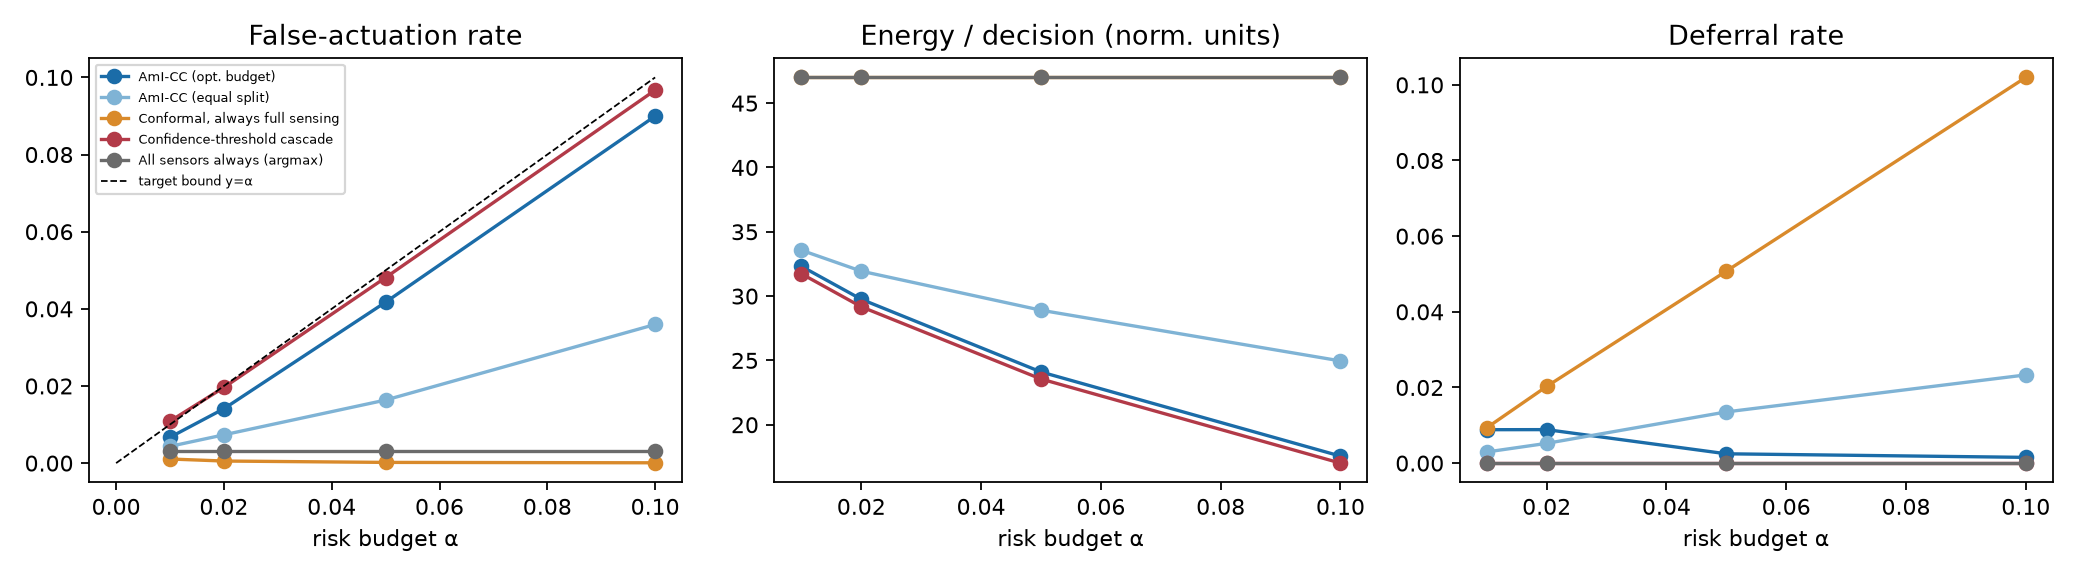
\includegraphics[width=\linewidth]{figures/fig_main.png}
\caption{Risk-budget sweep: false-actuation rate, energy and deferral rate (30 seeds).}
\end{figure}

\textbf{Robustness to occupant shift ($\alpha=0.05$).} The exchangeability assumption fails when test occupants are more heterogeneous than calibration occupants, and the bound is then exceeded (Table~\ref{tab:shift}). On-site recalibration with 800 labelled samples from the new environment restores it, at the price of more deferrals (the system safely asks more often).

\begin{table}[H]\centering\small
\caption{Occupant-shift robustness of AmI-CC (false-actuation rate, $\alpha=0.05$).}\label{tab:shift}
\begin{tabular}{@{}c c c c@{}}
\toprule
Shift severity & FA, calibrated pre-deployment & FA, + on-site recalibration (800 labelled) & Deferral after recal.\\ \midrule
$\times 1.0$ & 0.042 & 0.044 & 0.00 \\
$\times 1.5$ & 0.062 & 0.041 & 0.02 \\
$\times 2.0$ & 0.092 & 0.035 & 0.07 \\
$\times 3.0$ & 0.178 & 0.027 & 0.32 \\
\bottomrule
\end{tabular}
\end{table}

\begin{figure}[H]\centering
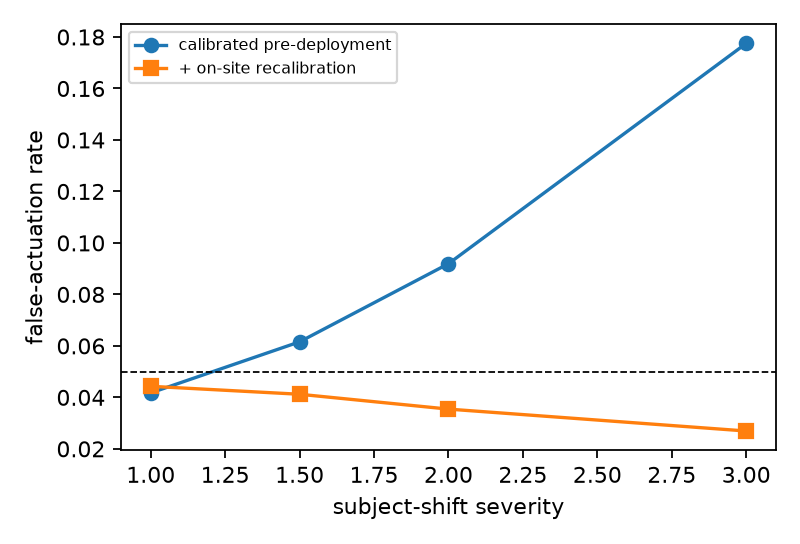
\includegraphics[width=0.55\linewidth]{figures/fig_shift.png}
\caption{Effect of occupant shift with and without on-site recalibration.}
\end{figure}

\textbf{Reproduce:} \texttt{python experiments/run\_experiments.py; python experiments/make\_figures.py; python tests/test\_cascade.py}. \textbf{Status:} results come from a simulator, not field data; a pilot on a public smart-home dataset / campus testbed is planned before TRL${\ge}4$ claims and is recommended before the journal submission.

\sect{9. What aspect(s) of the invention need(s) protection?}
\textbf{Independent claim 1 (method):} controlling actuation in an ambient IoT system, comprising: powering a first sensing tier; computing with a first classifier a conformal prediction set of candidate intents whose threshold is calibrated to a first miscoverage level $\alpha_1$; actuating if the set is a singleton, and otherwise powering a higher-energy tier and repeating; deferring if the last-tier set is not a singleton; wherein the miscoverage levels satisfy $\sum_t\alpha_t\le\alpha$, a predetermined actuation-risk budget, and are selected by minimising an objective comprising expected sensing energy on a data split disjoint from the split used to calibrate the thresholds.

\textbf{Dependent aspects:} (2) objective includes a deferral (user-interruption) cost $\lambda$; (3) grid/convex search of the allocation; (4) per-tier classifiers on cumulative features; (5) on-site recalibration from user overrides when a drift detector fires, deferring more often to preserve the bound; (6) tiers comprising PIR/door/light $\to$ plug-power/audio/BLE $\to$ camera/mmWave, so privacy-intrusive sensors are powered only on ambiguity; (7) class-conditional (per-action criticality) budgets [\emph{not yet validated}]; (8) system and (9) non-transitory medium claims. \emph{Technical effect emphasised for eligibility (e.g.\ Indian Patents Act s.3(k); 35~USC \S101): reduced power consumption of sensor hardware and a bounded rate of erroneous physical actuation.}

\sect{10. What is the Technology Readiness Level of your invention? (tick the appropriate TRL)}
\footnotesize
\begin{tabularx}{\linewidth}{@{}*{9}{>{\raggedright\arraybackslash}X}@{}}
\toprule
\multicolumn{3}{c}{\textbf{Research}} & \multicolumn{3}{c}{\textbf{Development}} & \multicolumn{3}{c}{\textbf{Deployment}}\\ \midrule
TRL 1 & TRL 2 & TRL 3 & TRL 4 & TRL 5 & TRL 6 & TRL 7 & TRL 8 & TRL 9\\
Basic principles observed & Technology concept formulated & \textbf{$\boxtimes$ Experimental proof of concept} & Technology validated in a lab & Validated in a relevant environment & Demonstrated in a relevant environment & System prototype in an operational environment & System complete and qualified & Actual system proven in an operational environment\\
\bottomrule
\end{tabularx}
\normalsize

Ticked: \textbf{TRL~3} (experimental proof of concept, simulation). Target: TRL~4 after a lab testbed run.

\begin{center}\footnotesize ---------------------- END OF THE DOCUMENT -----------------------------\end{center}
\end{document}
